\Def Хроматическое число пространста
$$\chi(\mathbb{R}^n)=\min\{\chi: (\mathbb{R}^n=V_1\! \sqcup\! ...\! \sqcup V_\chi)\! \wedge\! (\forall i \forall \vec{x}, \vec{y} \in V_i(\rho(\vec{x}, \vec{y}) \neq 1))\}$$

\Def Дистанционный граф $-$ граф $G(\mathbb{R}^n, E)$, где $E = \{ (\vec{x}, \vec{y}): \rho(\vec{x}, \vec{y})=1 \}$

\underline{Связь с дистанционным графом}: Хроматическое число $\mathbb{R}^n$ равно хроматическому числу дистанционного графа $\mathbb{R}^n$.

\underline{Простая оценка конечности}: $\chi(\mathbb{R}^n) \leqslant (4 \sqrt{n})^n$.
\Proof Выделяем квадратный брус со стороной 2 и делим его на квадратные брусы со стороной $\frac{1}{2\sqrt{n}}$. Тогда вдоль одной грани лежит $4 \sqrt{n}$ кубиков, а значит, во всём кубе находится $(4 \sqrt{n})^{n}$ кубиков. Красим каждый из них в свой цвет. Так максимальное расстояние в маленьком кубе - его главная диагональ длиной 1/2, то внутри одного кубика тоже не будет одноцветных точек на расстоянии 1. Значит, внутри одного большого куба раскраска корректная, а дальше мы можем замостить простарнство такими кубами, не меняя их ориентацию, и центры одноцветных кубиков будут ра расстоянии 2, а даже если грубо оценить их самые близкие наиобольшими расстояниями внутри, то они будут удалены больше чем на $2 - 1/2 \cdot 2=1$. Значит, раскраска пространства корректна. \EndProof

\underline{Известные оценки(б/д)}: \\
$-$ $\chi(\mathbb{R}^3) \leqslant 15$ \\
$-$ $\chi(\mathbb{R}^4) \leqslant 54$ \\
$-$ $\chi(\mathbb{R}^n) \leqslant (3 + \overline{\overline{o}}(1))^n$ \\
$-$ $\chi(\mathbb{R}^n) \geqslant \chi(G(n, 3, 1)) \geqslant \frac{C^3_n}{m(n, 3, 1)} \geqslant \frac{C^3_n}{n} \sim \frac{n^2}{6}$ \\
$-$ $\chi(\mathbb{R}^n) \geqslant \left(\frac{1+\sqrt{2}}{2} +  \overline{\overline{o}}(1) \right)^n$

\underline{Примеры}: \\
$-$ $\chi(\mathbb{R}^1)=2$: покраска полуинтервалами $[n, n+1)$; \\
$-$ $\chi(\mathbb{R}^2) \in [5, 7] \cap \mathbb{Z}$: оценка на мин. 4 $-$ веретено Мозера или граф Голомба, оценка на макс. 7 $-$ шестиугольники со стороной 0,4, оценка на мин. 5 $-$ пример Обри ди Брейна; \\

\begin{center}
    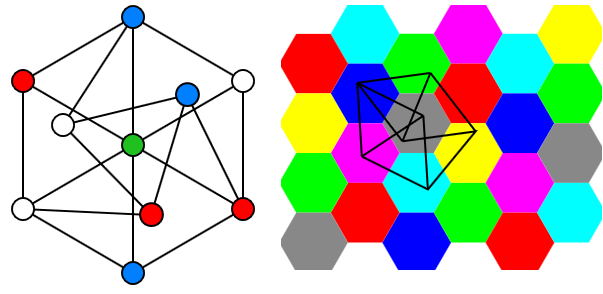
\includegraphics[scale=0.4]{images/Chromatic_plane.png}
\end{center}